\chapter{Results}
\label{cha:results}
In this chapter, two mobile subscriber trajectories will be presented that have been generated using the developed system. The generated trajectories cover semi-rural and urban areas, which allows evaluating the approach for different scenarios. All results are fully reproducible in case the same subscriber and coverage predictions are used.
\section{Example 1}
The first example covers a semi-rural region. A semi-rural region consist of a rural and an urban area. The following trajectory was recorded on Monday, 26 March 2012. At 08:08:29 in the morning the subscriber established a call. The duration of the call was 7 minutes and 36 seconds.  During the call the subscriber traversed the highway A7 from Linz\footnote{GPS position of call establishment Latitude: 48.28086955 Longitude:	14.30415398 \url{http://osm.org/go/0JhMzsg9l-?m=}} to Engerwitzdorf\footnote{GPS position of call termination Latitude: 48.3381025 Longitude:	14.4125565 \url{http://osm.org/go/0JhP~5vT--?m=}}. Between the call establishment and call termination the mobile station was connected to 22 transmitters which resulted in 21 handover events. Figure~\ref{fig:563overview} illustrates the traversed route as well as the estimated handover position for both the network planning tool coverage~\ref{fig:563coverage} and the Voronoi diagrams coverage~\ref{fig:563voronoi}.

%\begin{figure}
%\begin{tabular}{cc}
%  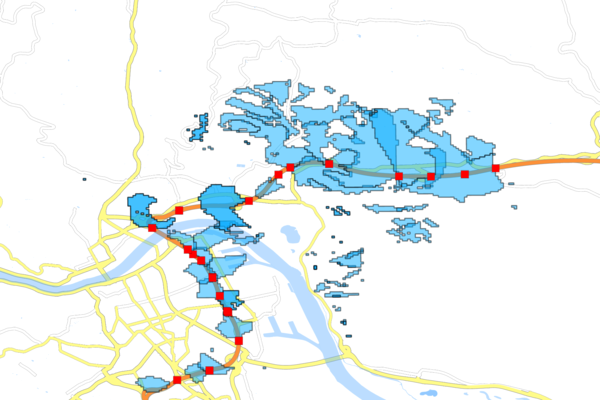
\includegraphics[width=65mm]{./images/563_Coverage_Handover}
%  &   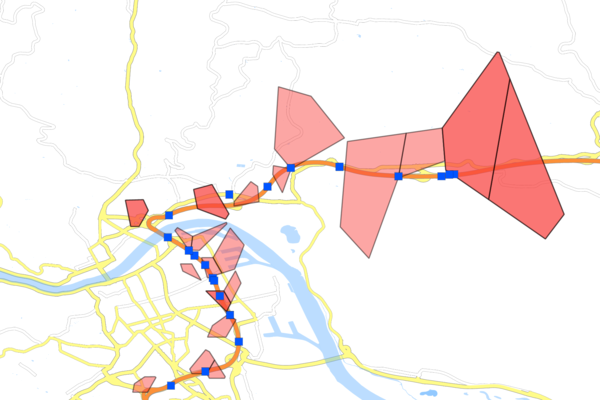
\includegraphics[width=65mm]{./images/563_Voronoi_Handover} \\
%(a)  & (b)  \\[6pt]
% 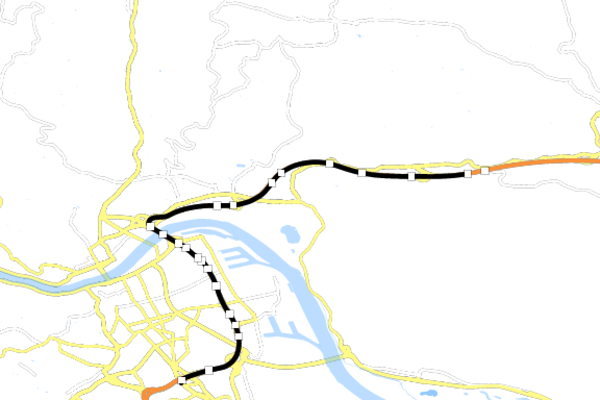
\includegraphics[width=65mm]{./images/563_Handover}
% &   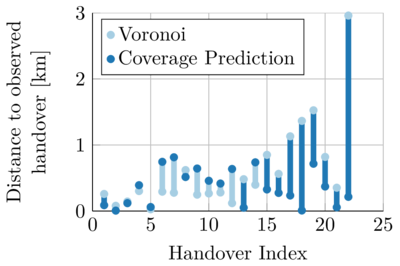
\includegraphics[width=65mm]{./images/563_predvorcomp} \\
%(c)  & (d)  \\[6pt]
%\end{tabular}
%\caption{Example 1 subscriber 563: (a) coverage prediction with network planning tool and estimated handover points, (b) Voronoi diagram coverage and estimated handover points, (c) recorded GPS route and observed handover points, (d) comparison of distance between estimated handover and observed handover}
%\label{fig:563overview}
%\end{figure}



\begin{figure}
	\centering
	\begin{subfigure}[b]{0.5\linewidth}
		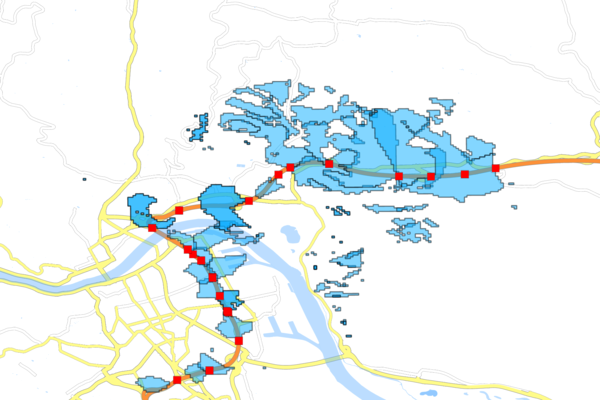
\includegraphics[width=\textwidth]{./images/563_Coverage_Handover}
		\caption{}
		\label{fig:563coverage}
	\end{subfigure}%
	~
	 %add desired spacing between images, e. g. ~, \quad, \qquad etc.
	%(or a blank line to force the subfigure onto a new line)
	\begin{subfigure}[b]{0.5\linewidth}
		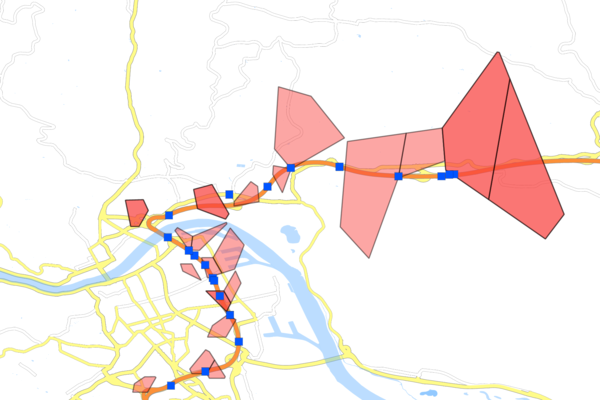
\includegraphics[width=\textwidth]{./images/563_Voronoi_Handover}
		\caption{}
		\label{fig:563voronoi}
	\end{subfigure}

	\begin{subfigure}[b]{0.5\linewidth}
			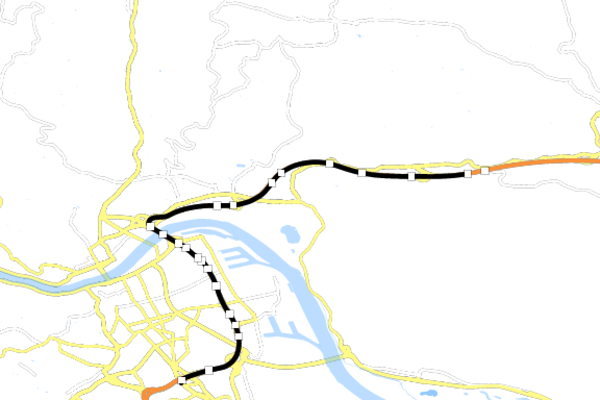
\includegraphics[width=\textwidth]{./images/563_Handover}
			\caption{}
			\label{fig:563handover}
		\end{subfigure}%
		~
		 %add desired spacing between images, e. g. ~, \quad, \qquad etc.
		%(or a blank line to force the subfigure onto a new line)
		\begin{subfigure}[b]{0.5\linewidth}
			\centering
%			\tikzsetnextfilename{563_predvorcomp}
		%	% This file was created by matlab2tikz v0.4.7 running on MATLAB 8.2.
% Copyright (c) 2008--2014, Nico Schlömer <nico.schloemer@gmail.com>
% All rights reserved.
% Minimal pgfplots version: 1.3
% 
% The latest updates can be retrieved from
%   http://www.mathworks.com/matlabcentral/fileexchange/22022-matlab2tikz
% where you can also make suggestions and rate matlab2tikz.
% 
%
% defining custom colors
\definecolor{mycolor1}{rgb}{0.12157,0.47059,0.70588}%
\definecolor{mycolor2}{rgb}{0.65098,0.80784,0.89020}%
%

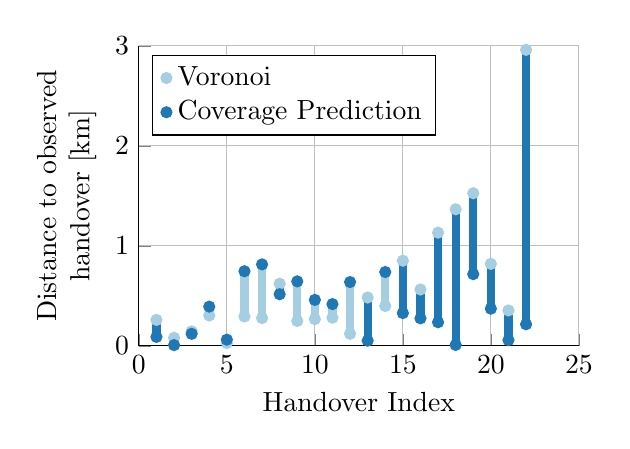
\begin{tikzpicture}

\begin{axis}[%
width=2.2in,
height=1.5in,
scale only axis,
xmin=0,
xmax=25,
xlabel={Handover Index},
ymin=0,
ymax=3,
xmajorgrids,
ymajorgrids,
ylabel style={align=center}, ylabel={Distance to observed\\handover [km]},
axis x line*=bottom,
axis y line*=left,
legend style={at={(0.03,0.97)},anchor=north west,draw=black,fill=white,legend cell align=left}
]
\addplot [color=mycolor1,solid,line width=3.0pt,forget plot]
  table[row sep=crcr]{1	0.259018648229545\\
1	0.0891149921062485\\
};
\addplot [color=mycolor1,solid,line width=3.0pt,forget plot]
  table[row sep=crcr]{2	0.0797827807909224\\
2	0.00719807672629999\\
};
\addplot [color=mycolor1,solid,line width=3.0pt,forget plot]
  table[row sep=crcr]{3	0.144328979813695\\
3	0.11981134044023\\
};
\addplot [color=mycolor2,solid,line width=3.0pt,forget plot]
  table[row sep=crcr]{4	0.303214980482706\\
4	0.391874747309698\\
};
\addplot [color=mycolor2,solid,line width=3.0pt,forget plot]
  table[row sep=crcr]{5	0.0273400999818614\\
5	0.0614465353921736\\
};
\addplot [color=mycolor2,solid,line width=3.0pt,forget plot]
  table[row sep=crcr]{6	0.293589904815724\\
6	0.745484009237662\\
};
\addplot [color=mycolor2,solid,line width=3.0pt,forget plot]
  table[row sep=crcr]{7	0.277796892878827\\
7	0.814326322320143\\
};
\addplot [color=mycolor1,solid,line width=3.0pt,forget plot]
  table[row sep=crcr]{8	0.620684025308691\\
8	0.515743821301441\\
};
\addplot [color=mycolor2,solid,line width=3.0pt,forget plot]
  table[row sep=crcr]{9	0.248469551426603\\
9	0.644388462148261\\
};
\addplot [color=mycolor2,solid,line width=3.0pt,forget plot]
  table[row sep=crcr]{10	0.267079515137835\\
10	0.458909692535503\\
};
\addplot [color=mycolor2,solid,line width=3.0pt,forget plot]
  table[row sep=crcr]{11	0.281221206930742\\
11	0.417008090587785\\
};
\addplot [color=mycolor2,solid,line width=3.0pt,forget plot]
  table[row sep=crcr]{12	0.120058778792591\\
12	0.637525807123021\\
};
\addplot [color=mycolor1,solid,line width=3.0pt,forget plot]
  table[row sep=crcr]{13	0.482668591082766\\
13	0.0513571194839525\\
};
\addplot [color=mycolor2,solid,line width=3.0pt,forget plot]
  table[row sep=crcr]{14	0.398331306743372\\
14	0.737778218182398\\
};
\addplot [color=mycolor1,solid,line width=3.0pt,forget plot]
  table[row sep=crcr]{15	0.851141896655434\\
15	0.32735177986664\\
};
\addplot [color=mycolor1,solid,line width=3.0pt,forget plot]
  table[row sep=crcr]{16	0.562950007374927\\
16	0.274928631737445\\
};
\addplot [color=mycolor1,solid,line width=3.0pt,forget plot]
  table[row sep=crcr]{17	1.13161564831271\\
17	0.235897510899756\\
};
\addplot [color=mycolor1,solid,line width=3.0pt,forget plot]
  table[row sep=crcr]{18	1.36532254757252\\
18	0.00888274629650682\\
};
\addplot [color=mycolor1,solid,line width=3.0pt,forget plot]
  table[row sep=crcr]{19	1.52569390282899\\
19	0.716690329740095\\
};
\addplot [color=mycolor1,solid,line width=3.0pt,forget plot]
  table[row sep=crcr]{20	0.81953085437581\\
20	0.371649721270948\\
};
\addplot [color=mycolor1,solid,line width=3.0pt,forget plot]
  table[row sep=crcr]{21	0.35366213246396\\
21	0.0571271279972839\\
};
\addplot [color=mycolor1,solid,line width=3.0pt,forget plot]
  table[row sep=crcr]{22	2.95963417791592\\
22	0.215560825161708\\
};
\addplot[only marks,mark=*,mark options={},color=mycolor2] plot table[row sep=crcr,]{1	0.259018648229545\\
2	0.0797827807909224\\
3	0.144328979813695\\
4	0.303214980482706\\
5	0.0273400999818614\\
6	0.293589904815724\\
7	0.277796892878827\\
8	0.620684025308691\\
9	0.248469551426603\\
10	0.267079515137835\\
11	0.281221206930742\\
12	0.120058778792591\\
13	0.482668591082766\\
14	0.398331306743372\\
15	0.851141896655434\\
16	0.562950007374927\\
17	1.13161564831271\\
18	1.36532254757252\\
19	1.52569390282899\\
20	0.81953085437581\\
21	0.35366213246396\\
22	2.95963417791592\\
};
\addlegendentry{Voronoi};

\addplot[only marks,mark=*,mark options={},color=mycolor1] plot table[row sep=crcr,]{1	0.0891149921062485\\
2	0.00719807672629999\\
3	0.11981134044023\\
4	0.391874747309698\\
5	0.0614465353921736\\
6	0.745484009237662\\
7	0.814326322320143\\
8	0.515743821301441\\
9	0.644388462148261\\
10	0.458909692535503\\
11	0.417008090587785\\
12	0.637525807123021\\
13	0.0513571194839525\\
14	0.737778218182398\\
15	0.32735177986664\\
16	0.274928631737445\\
17	0.235897510899756\\
18	0.00888274629650682\\
19	0.716690329740095\\
20	0.371649721270948\\
21	0.0571271279972839\\
22	0.215560825161708\\
};
\addlegendentry{Coverage Prediction};

\end{axis}
\end{tikzpicture}%
			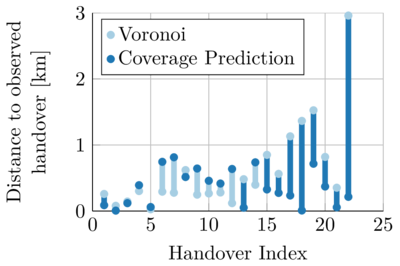
\includegraphics[width=\textwidth]{./images/563_predvorcomp}
			\caption{}
			\label{fig:563distcomp}
		\end{subfigure}

	\caption{Example 1: (a) coverage prediction with network planning tool and estimated handover points, (b) Voronoi diagram coverage and estimated handover points, (c) recorded GPS route and observed handover points, (d) comparison of distance between estimated handover and observed handover}\label{fig:563overview}
\end{figure}


\subsubsection{Route}
To estimate the subscribers route, 20 random start and end positions within the coverage area of the first and last cell were used. The random positions were derived from a probability density function that was generated by the population density in the area as described in Section~\ref{sec:startandend}. Table~\ref{tab:563route} depicts the metrics used to choose the best approximation. This metrics are the time-ratio between the journey time and the time it takes to traverse the route as well as the summed square of distances between the route and the centroids of the involved cell sites. An illustration of all computed routes can be found in Figure~\ref{fig:563_routes}. The time-ration in conjunction with the squared sum of distances between the route and each coverage area allows the system to choose the best approximated route. In case of subscriber 563 the route with time-ratio $1.00$ and $\sum {d}_{i}^{2}=0.35$ was picked. To compare the estimated route with the real route recorded with GPS the Hausdorff metric was used. The Hausdorff metric for the chosen route  compared with the actual route was $0.990138 $. That means that the maximum distance between the chosen route and the actual route was very small. Thus, the similarity of  both routes is high. A second metric which takes the continuity of both routes into account is the Frechet distance. A Frechet distance of $0$ means that both routes are identical. Therefore, the smaller the Frechet distance is, the higher is the similarity. The computed Frechet distance for the estimated route was $0.0134$. Even if the estimated route corresponds to the actual route -- recorded with GPS -- the Frechet distance is not $0$. This is due to the fact that GPS introduces an error which can lead to a deviation.
\begin{figure}
\centering
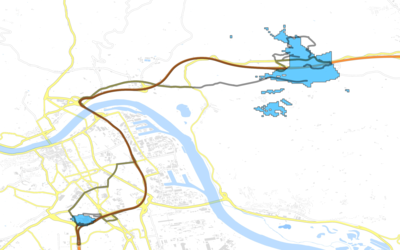
\includegraphics[width=0.7\linewidth]{./images/563_routes}
\caption{Example 1: Illustration of 20 routes with different start and end position}
\label{fig:563_routes}
\end{figure}


\begin{table}
\centering
\begin{tabular}{l|l|l|l}
Time-ratio & Mean distance $\overline{d_i}$ & Variance $\mathrm{Var}[d_i]$& $\sum {d}_{i}^{2}$ \\
\hline
0.96 & 0.09 & 0.03 & 1.38 \\
0.97 & 0.04 & 0.01 & 0.36 \\
0.97 & 0.09 & 0.03 & 1.39 \\
0.99 & 0.04 & 0.01 & 0.35 \\
0.99 & 0.04 & 0.01 & 0.35 \\
0.99 & 0.09 & 0.03 & 1.38 \\
\textbf{1.00} & \textbf{0.04 }& \textbf{0.01} & \textbf{0.35} \\
1.00 & 0.04 & 0.01 & 0.35 \\
1.01 & 0.05 & 0.01 & 0.42 \\
1.01 & 0.09 & 0.03 & 1.38 \\
1.02 & 0.04 & 0.01 & 0.36 \\
1.03 & 0.09 & 0.03 & 1.38 \\
1.03 & 0.09 & 0.03 & 1.38 \\
1.04 & 0.04 & 0.01 & 0.36 \\
1.04 & 0.09 & 0.03 & 1.38 \\
1.05 & 0.04 & 0.01 & 0.35 \\
1.05 & 0.09 & 0.03 & 1.38 \\
1.08 & 0.07 & 0.03 & 1.18 \\
1.10 & 0.07 & 0.03 & 1.18 \\
1.10 & 0.07 & 0.03 & 1.18
\end{tabular}
\caption{Example 1:  Statistical comparison of the 20 computed routes}
\label{tab:563route}
\end{table}
\subsubsection{Handover}
After the subscriber route was approximated handover points were estimated. The estimation was done for both the network coverage prediction and the Voronoi diagram coverage. Figure~\ref{fig:563distcomp} shows a comparison of distances between the observed handover position and the estimated handover position for both the network coverage prediction and Voronoi diagram coverage. It can be seen that the handover estimation done with Voronoi diagram coverage performed better than the network coverage prediction for the first half of the route. On the other hand the network coverage prediction performed better in the second half of the route.
\subsubsection{Velocity}
The velocity for each segment has been calculated with the approach introduced in Section~\ref{sec:velocity}. Due to deviation between the observed handover position and the estimated handover position a velocity over-run and under-run has happened at the beginning and the end of the trajectory. The velocity over-run was eliminated with the adaption algorithm presented in Section~\ref{sec:adaption}. The effect of the adaption can be seen in Figure~\ref{fig:563velocity}. The first figure shows a comparison of the observed velocity with the estimated velocity when no adaption has been done. On the other hand, the second figure depicts the effect of the adaption algorithm. The velocity overrun that is visible in the first figure between second 310 and 330 has been eliminated.
\begin{figure}
	\centering
	\begin{subfigure}[b]{\textwidth}
		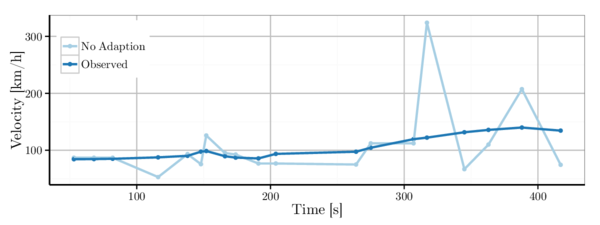
\includegraphics[width=\textwidth]{./images/563_velocityNoAdapt}
		\caption{}
		\label{fig:563_velocityNoAdapt}
	\end{subfigure}%

	 %add desired spacing between images, e. g. ~, \quad, \qquad etc.
	%(or a blank line to force the subfigure onto a new line)
	\begin{subfigure}[b]{\textwidth}
		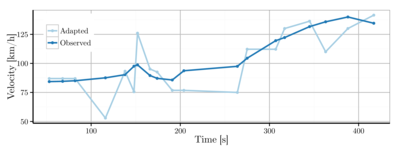
\includegraphics[width=\textwidth]{./images/563_velocityAdapt}
		\caption{}
		\label{fig:563_velocityAdapt}
	\end{subfigure}
	\caption{Example 1: Comparison of velocity (a) without adaption  and (b) with adaption}\label{fig:563velocity}
\end{figure}

\section{Example 2}
The second example depicts an urban scenario. The trajectory for this example was recorded on Saturday, 26 May 2012. The subscriber established a call at 12:12:57. The duration of the call was 6 minutes and 33 seconds. During the call the subscriber drove from Linz-Urfahr\footnote{GPS position of call establishment Latitude:48.31600 Longitude:14.29023 \url{http://osm.org/go/0JhNlzhh--?m=}} over the minor road network and the highway A7 to Linz-Bindermichl\footnote{GPS position of call termination Latitude:48.2814 Longitude:14.3029 \url{http://osm.org/go/0JhMzuVj?m=}}. Between the call establishment and call termination the mobile station was connected to 17 transmitter which resulted in 16 handover events. The traversed route and the observed handover positions are illustrated in Figure~\ref{fig:1058_handover}. The estimated handover positions for both the network planning tool coverage and the Voronoi diagram coverage are depicted in Figure~\ref{fig:1058_coverage} and \ref{fig:1058_voronoi}.
\begin{figure}
	\centering
	\begin{subfigure}[b]{0.5\linewidth}
		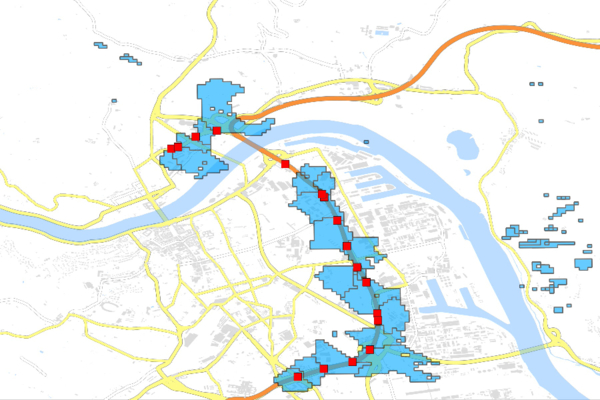
\includegraphics[width=\textwidth]{./images/1058_Coverage_Handover}
		\caption{}
		\label{fig:1058_coverage}
	\end{subfigure}%
	~
	 %add desired spacing between images, e. g. ~, \quad, \qquad etc.
	%(or a blank line to force the subfigure onto a new line)
	\begin{subfigure}[b]{0.5\linewidth}
		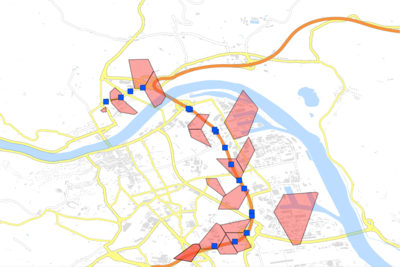
\includegraphics[width=\textwidth]{./images/1058_Voronoi_Handover}
		\caption{}
		\label{fig:1058_voronoi}
	\end{subfigure}

	\begin{subfigure}[b]{0.5\linewidth}
			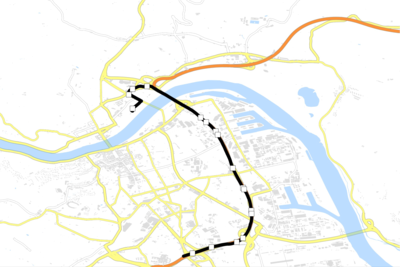
\includegraphics[width=\textwidth]{./images/1058_Handover}
			\caption{}
			\label{fig:1058_handover}
		\end{subfigure}%
		~
		 %add desired spacing between images, e. g. ~, \quad, \qquad etc.
		%(or a blank line to force the subfigure onto a new line)
		\begin{subfigure}[b]{0.5\linewidth}
		%\pgfplotsset{width=0.8\linewidth,compat=newest}
%		\tikzsetnextfilename{1058_predvorcomp}

	%	% This file was created by matlab2tikz v0.4.7 running on MATLAB 8.2.
% Copyright (c) 2008--2014, Nico Schlömer <nico.schloemer@gmail.com>
% All rights reserved.
% Minimal pgfplots version: 1.3
% 
% The latest updates can be retrieved from
%   http://www.mathworks.com/matlabcentral/fileexchange/22022-matlab2tikz
% where you can also make suggestions and rate matlab2tikz.
% 
%
% defining custom colors
\definecolor{mycolor1}{rgb}{0.12157,0.47059,0.70588}%
\definecolor{mycolor2}{rgb}{0.65098,0.80784,0.89020}%
%
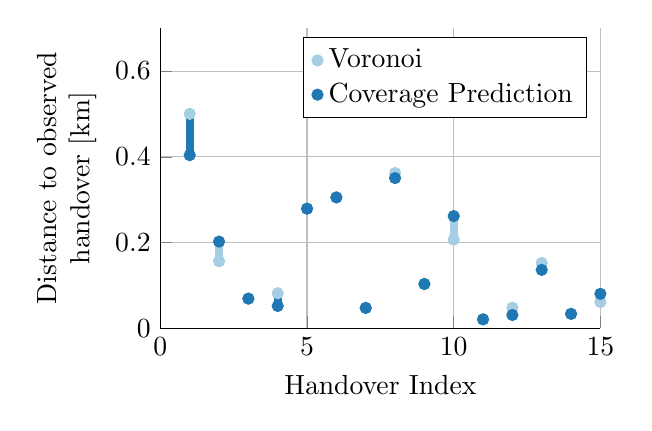
\begin{tikzpicture}

\begin{axis}[%
width=2.2in,
height=1.5in,
scale only axis,
xmin=0,
xmax=15,
xlabel={Handover Index},
ymin=0,
ymax=0.7,
xmajorgrids,
ymajorgrids,
ylabel style={align=center}, ylabel={Distance to observed\\handover [km]},
axis x line*=bottom,
axis y line*=left,
legend pos=north east,
legend style={anchor=north east,draw=black,fill=white,legend cell align=left}
]
\addplot [color=mycolor1,solid,line width=3.0pt,forget plot]
  table[row sep=crcr]{1	0.500266767072031\\
1	0.403833380195351\\
};
\addplot [color=mycolor2,solid,line width=3.0pt,forget plot]
  table[row sep=crcr]{2	0.156180660806584\\
2	0.2021357385342\\
};
\addplot [color=mycolor1,solid,line width=3.0pt,forget plot]
  table[row sep=crcr]{3	0.06904818124207\\
3	0.0690175773659844\\
};
\addplot [color=mycolor1,solid,line width=3.0pt,forget plot]
  table[row sep=crcr]{4	0.0816747782959422\\
4	0.0518977374762014\\
};
\addplot [color=mycolor1,solid,line width=3.0pt,forget plot]
  table[row sep=crcr]{5	0.278895223663847\\
5	0.278887325365906\\
};
\addplot [color=mycolor2,solid,line width=3.0pt,forget plot]
  table[row sep=crcr]{6	0.305204360585667\\
6	0.30521002814451\\
};
\addplot [color=mycolor2,solid,line width=3.0pt,forget plot]
  table[row sep=crcr]{7	0.047350066258318\\
7	0.0473793586876721\\
};
\addplot [color=mycolor1,solid,line width=3.0pt,forget plot]
  table[row sep=crcr]{8	0.362190942224447\\
8	0.350325971769639\\
};
\addplot [color=mycolor2,solid,line width=3.0pt,forget plot]
  table[row sep=crcr]{9	0.103163569468859\\
9	0.10320836001024\\
};
\addplot [color=mycolor2,solid,line width=3.0pt,forget plot]
  table[row sep=crcr]{10	0.206639412861688\\
10	0.261690187813169\\
};
\addplot [color=mycolor2,solid,line width=3.0pt,forget plot]
  table[row sep=crcr]{11	0.0206671106886966\\
11	0.0206780058925156\\
};
\addplot [color=mycolor1,solid,line width=3.0pt,forget plot]
  table[row sep=crcr]{12	0.0477743686694561\\
12	0.0308233923865931\\
};
\addplot [color=mycolor1,solid,line width=3.0pt,forget plot]
  table[row sep=crcr]{13	0.152222464957132\\
13	0.136157615534261\\
};
\addplot [color=mycolor2,solid,line width=3.0pt,forget plot]
  table[row sep=crcr]{14	0.0334508635747766\\
14	0.0334703841921082\\
};
\addplot [color=mycolor2,solid,line width=3.0pt,forget plot]
  table[row sep=crcr]{15	0.061112433940154\\
15	0.080214107952751\\
};
\addplot[only marks,mark=*,mark options={},color=mycolor2] plot table[row sep=crcr,]{1	0.500266767072031\\
2	0.156180660806584\\
3	0.06904818124207\\
4	0.0816747782959422\\
5	0.278895223663847\\
6	0.305204360585667\\
7	0.047350066258318\\
8	0.362190942224447\\
9	0.103163569468859\\
10	0.206639412861688\\
11	0.0206671106886966\\
12	0.0477743686694561\\
13	0.152222464957132\\
14	0.0334508635747766\\
15	0.061112433940154\\
};
\addlegendentry{Voronoi};

\addplot[only marks,mark=*,mark options={},color=mycolor1] plot table[row sep=crcr,]{1	0.403833380195351\\
2	0.2021357385342\\
3	0.0690175773659844\\
4	0.0518977374762014\\
5	0.278887325365906\\
6	0.30521002814451\\
7	0.0473793586876721\\
8	0.350325971769639\\
9	0.10320836001024\\
10	0.261690187813169\\
11	0.0206780058925156\\
12	0.0308233923865931\\
13	0.136157615534261\\
14	0.0334703841921082\\
15	0.080214107952751\\
};
\addlegendentry{Coverage Prediction};

\end{axis}
\end{tikzpicture}%

			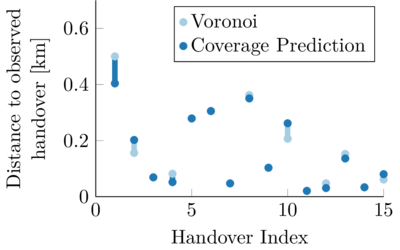
\includegraphics[width=\textwidth]{./images/1058_predvorcomp}
			\caption{}
			\label{fig:1058_distcomp}
		\end{subfigure}

	\caption{Example 2: (a) coverage prediction with network planning tool and estimated handover points, (b) Voronoi diagram coverage and estimated handover points, (c) recorded GPS route and observed handover points, (d) comparison of distance between estimated handover and observed handover}\label{fig:1058overview}
\end{figure}
\subsubsection{Route}
The same technique described in example one was used to estimate the subscriber route. In Table~\ref{tab:1058route} all estimated routes are shown; the most suitable was highlighted. The most suitable route in this example  had a time-ratio of  $0.97$ and a sum square distance of $\sum {d}_{i}^{2}=0.40$. The Hausdorff metric and Frechet distance was used again to measure the similarity of the most suited route and the actual traveled route. Figure~\ref{fig:1058_routes} illustrates the 20 routes which have been computed between the estimated start and end position. The Hausdorff metric was $0.933091$ which indicates that there has been a deviation with the estimated start and end position and the actual one. However, the Frechet distance was  $0.0034$ which means that the geometry of both routes is very similar.
\begin{figure}
\centering
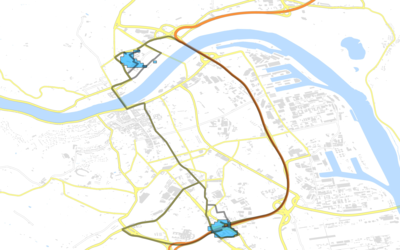
\includegraphics[width=0.7\linewidth]{./images/1058_routes}
\caption{Example 2: Illustration of 20 routes with different start and end position}
\label{fig:1058_routes}
\end{figure}

\begin{table}
\centering
\begin{tabular}{l|l|l|l}
Time-ratio & Mean distance $\overline{d_i}$ & Variance $\mathrm{Var}[d_i]$& $\sum {d}_{i}^{2}$ \\
\hline
0.85 & 0.82 & 0.39 & 19.77 \\
0.87 & 0.80 & 0.40 & 19.25 \\
0.90 & 0.78 & 0.43 & 19.13 \\
0.91 & 0.09 & 0.02 & 0.50 \\
0.93 & 0.78 & 0.41 & 19.08 \\
0.95 & 0.80 & 0.41 & 19.50 \\
0.95 & 0.80 & 0.40 & 19.30 \\
0.97 & 0.19 & 0.08 & 2.03 \\
0.97 & 0.78 & 0.41 & 18.88 \\
\textbf{0.97} & \textbf{0.07} &\textbf{0.02} &\textbf{0.40} \\
0.98 & 0.77 & 0.41 & 18.46 \\
1.01 & 0.76 & 0.41 & 18.34 \\
1.11 & 0.86 & 0.40 & 21.12 \\
1.12 & 0.83 & 0.40 & 20.24 \\
1.12 & 0.86 & 0.41 & 21.32 \\
1.13 & 0.83 & 0.41 & 20.44 \\
1.14 & 0.80 & 0.41 & 19.59 \\
1.17 & 0.79 & 0.41 & 19.06 \\
1.17 & 0.79 & 0.41 & 19.06 \\
1.17 & 0.84 & 0.40 & 20.62
\end{tabular}
\caption{Example 2: Comparison of time-ration, mean, variance and sum square of the 20 computed route}
\label{tab:1058route}
\end{table}
\subsubsection{Handover}
In this example the handover estimation with network coverage prediction was more accurate than with Voronoi diagram prediction. This, however, is interesting as it is the opposite of the first example. In the first example Voronoi diagrams performed better in the urban area than the network coverage prediction. The reason for this can be that the subscriber was connected to a different set of cells while driving the same road network. Figure~\ref{fig:1058_distcomp} depicts the distance difference between the observed handover position and the one estimated with both Voronoi diagram coverage and network coverage prediction.
\subsubsection{Velocity}
Similar to the first example there was a deviation of estimated and observed handover positions. This deviation introduced an error which led to an increase in speed for the segment where the deviation happened. In Figure~\ref{fig:1058_velocityNoAdapt} the speed increase is visible as four spikes. The adaption algorithm was used to remove this speed over-runs. The result of the adaption algorithm can be seen in Figure~\ref{fig:1058_velocityAdapt}.



\begin{figure}
	\centering
	\begin{subfigure}[b]{\textwidth}
		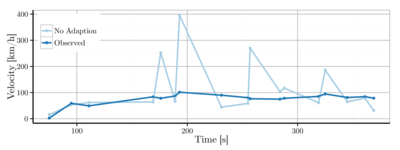
\includegraphics[width=\textwidth]{./images/1058_velocityNoAdapt}
		\caption{}
		\label{fig:1058_velocityNoAdapt}
	\end{subfigure}%

	 %add desired spacing between images, e. g. ~, \quad, \qquad etc.
	%(or a blank line to force the subfigure onto a new line)
	\begin{subfigure}[b]{\textwidth}
		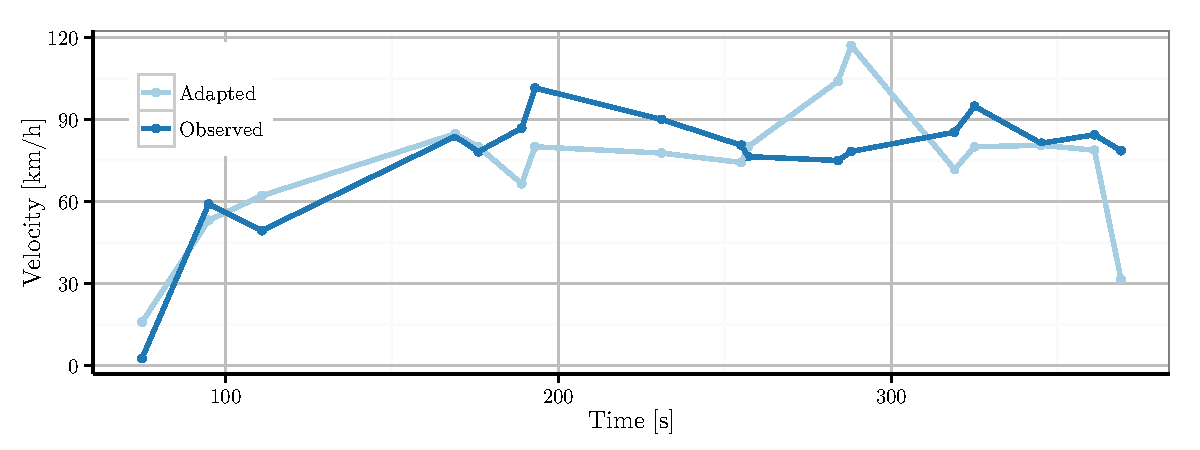
\includegraphics[width=\textwidth]{./images/1058_velocityAdapt}
		\caption{}
		\label{fig:1058_velocityAdapt}
	\end{subfigure}
	\caption{Example 2: Comparison of velocity (a) without adaption  and (b) with adaption}\label{fig:1058velocity}
\end{figure}


